\documentclass[tikz, border=10pt]{standalone}
\usepackage{pgfplots}
\pgfplotsset{compat=1.18}

\begin{document}
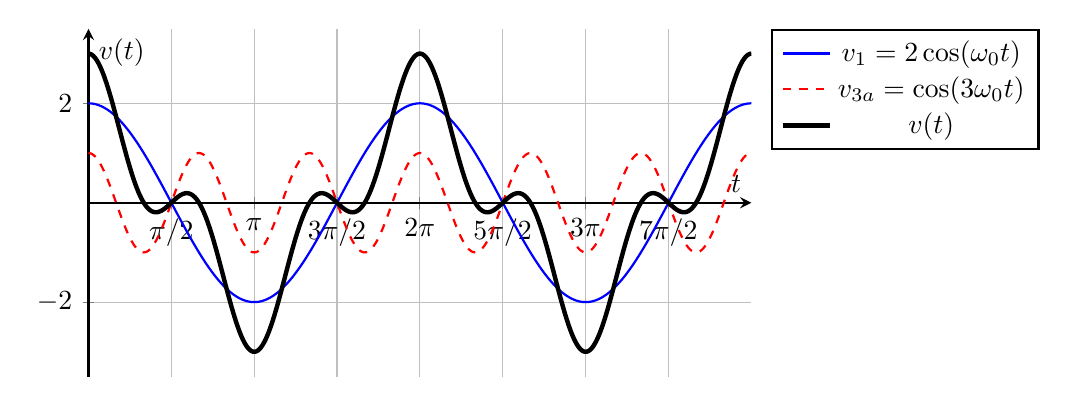
\begin{tikzpicture}
    \begin{axis}[
        width=10cm, height=6cm,
        axis lines=middle,
        xlabel={$t$}, ylabel={$v(t)$},
        ymin=-3.5, ymax=3.5,
        xmin=0, xmax=4*pi,
        xtick={0, 1.57, 3.14, 4.71, 6.28, 7.85, 9.42, 10.99, 12.57},
        xticklabels={0, $\pi/2$, $\pi$, $3\pi/2$, $2\pi$, $5\pi/2$, $3\pi$, $7\pi/2$, $4\pi$},
        legend pos=outer north east,
        grid=both,
        samples=400,
        domain=0:4*pi,
        thick
    ]
        % Fundamental v1 = 2cos(w0t)
        \addplot[blue] {2*cos(deg(x))};
        \addlegendentry{$v_1 = 2\cos(\omega_0 t)$}
        
        % Third harmonic v3a = cos(3w0t)
        \addplot[red, dashed] {cos(deg(3*x))};
        \addlegendentry{$v_{3a} = \cos(3\omega_0 t)$}
        
        % Summation
        \addplot[black, ultra thick] {2*cos(deg(x)) + cos(deg(3*x))};
        \addlegendentry{$v(t)$}
    \end{axis}
\end{tikzpicture}
\end{document}
